\section{Database and Annotation}
\subsection{Statistics and protocols}
MSU-PID includes two plant databases: Arabidopsis and Bean.
The statistic information of these two databases are summarised in Tab.~\ref{tab:stat}.
The images were acquired every hour.
As there is no light at night, plants can not be captured in fluorescence and RGB color images while IR and depth cameras can still capture plants.
Therefore, in order to make it consistent, we release images captured only in day time, which are $16$ images per day for Arabidopsis and $14$ for bean for all four sensors.

\begin{table*}
\begin{center}
\caption{Summary of Arabidopsis and Bean databases.}
\label{tab:stat}
\begin{tabular}{c|c|c|c|c|c}
      \hline
      % after \\: \hline or \cline{col1-col2} \cline{col3-col4} ...
      Database     & Subjects & Days & Images/Day & Total Images & Annotated Images \\
      \hline
      Arabidopsis &  16      &  9   &     16     &     2304     &       576    \\
      %\hline
      Bean        &   5      &  5   &     14     &     350      &       175 \\
      \hline
\end{tabular}
\end{center}
\end{table*}

The two databases differs in plant resolutions.
As shown in Fig~\ref{fig:rawIm},  we grow a single bean plant while a whole tray of Arabidopsis are grown at the same time.
Therefore, the resolution of each Arabidopsis plant is much lower than that of a bean plant.
We manually crop $16$ Arabidopsis plants, which have been captured by all four sensors.
Table~\ref{tab:resolution} summaries the resolution of each plant in all four channels.

\begin{figure*}
\begin{centering}
\begin{tabular}{c c}
%\begin{tabular}{@{}c@{} c@{}}
%\begin{tabular}{lllllllll}
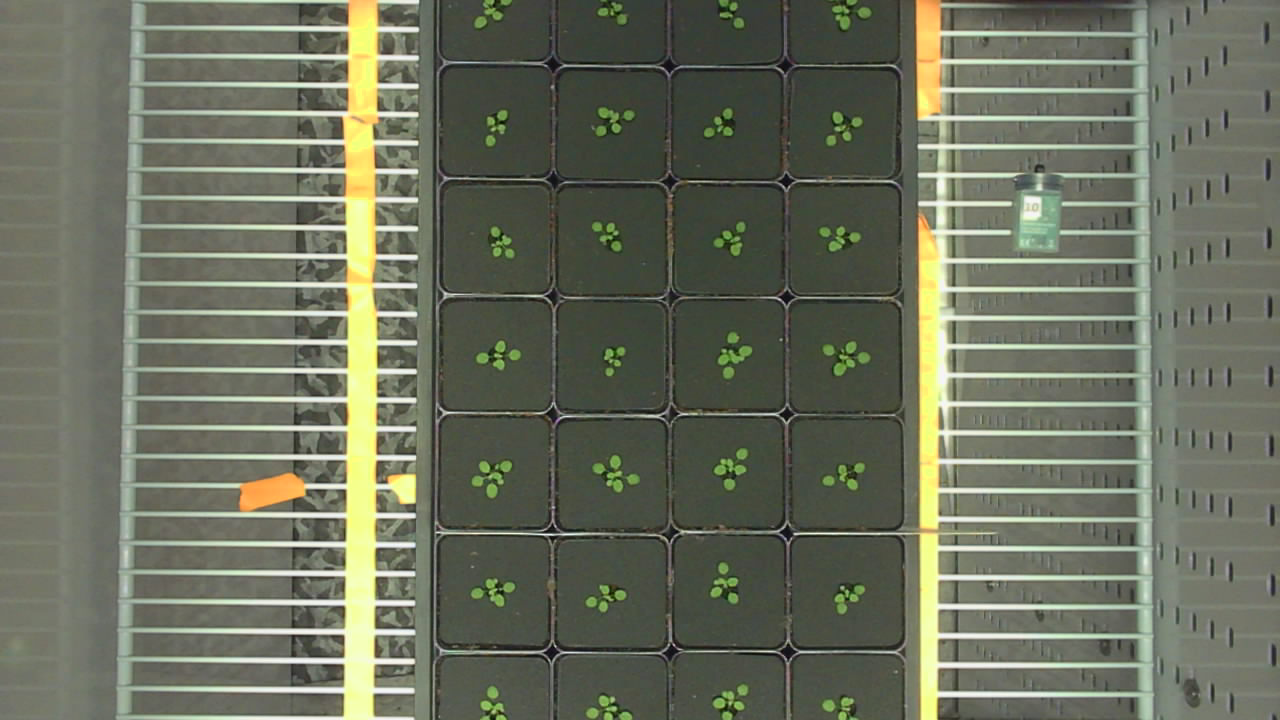
\includegraphics[width=.45\textwidth]{Figures/rawImages/a.png}&
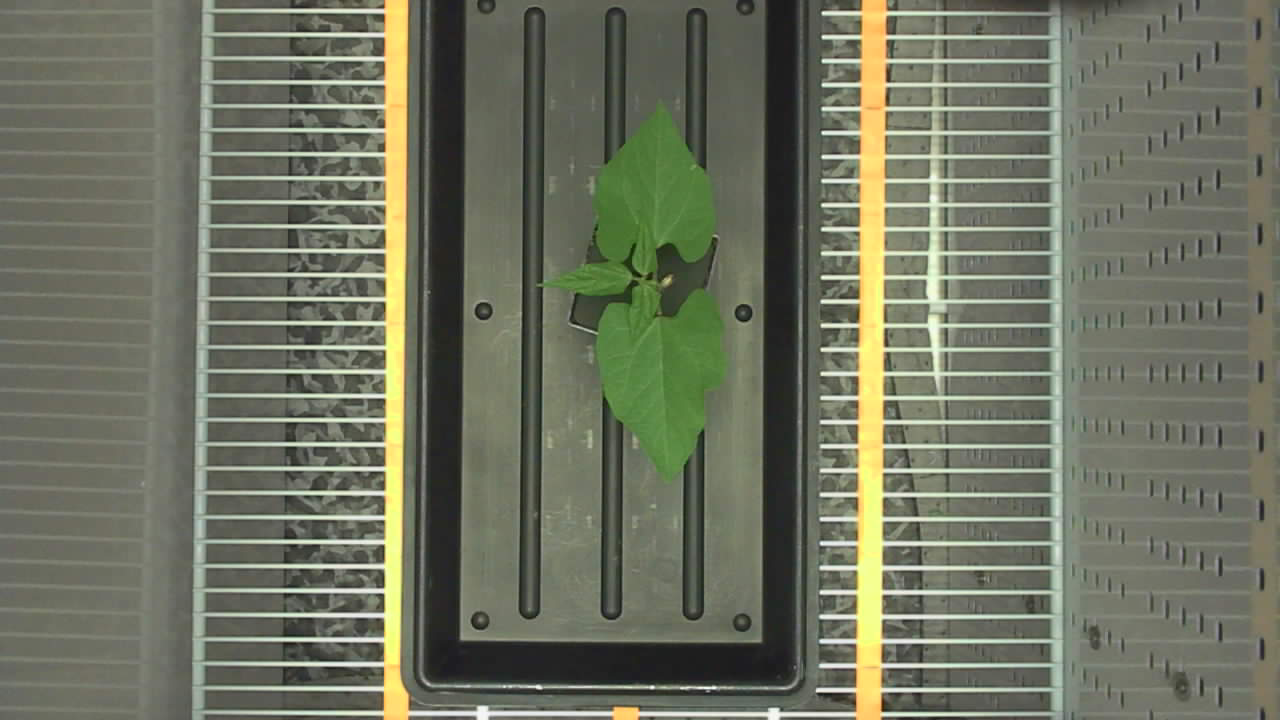
\includegraphics[width=.45\textwidth]{Figures/rawImages/b.png}\\
  Arabidopsis & Bean \\
\end{tabular}
\caption{Color images of Arabidopsis and bean plants. }
\label{fig:rawIm}
\end{centering}
\end{figure*}

\begin{table*}
\begin{center}
\caption{Plant resolution of Arabidopsis and Bean databases.}
\label{tab:resolution}
\begin{tabular}{c|c|c|c|c}
      \hline
      % after \\: \hline or \cline{col1-col2} \cline{col3-col4} ...
      Database     & Fluorescence       & IR        & RGB      & Depth     \\
      \hline
      Arabidopsis &  ~240$\times$240 &  ~240$\times$240 & ~120$\times$120  & NA  \\
      %\hline
      Bean        & 1360$\times$1024 & 1360$\times$1024 & 1280$\times$720 & 320$\times$240    \\
      \hline
\end{tabular}
\end{center}
\end{table*}


As shown in Tab.~\ref{tab:database}, MSU-PID can be used for leaf segmentation, leaf alignment, leaf tracking, and leaf counting.
To facilitate future research, we separate the database into training set and testing set.
$40\%$ of the data is used for training and $60\%$ for testing.
Specifically, $6$ plants of Arabidopisis and $2$ plants of bean are selected for training.
We will provide training and testing data in different folders.
For fair comparison, both supervised learning and unsupervised learning methods should evaluate the performance on the training and testing sets separately.
The evaluation metrics will be discussed in Sec.~\ref{sec:baseline}.



\subsection{Manual annotations}
Part of the database is manually annotated to provide ground truth tip locations, leaf segmentation results and leaf consistency overtime.
Tip locations are saved in a TXT file for each frame.
Leaf segmentation results are stored in a PNG image for each frame with one color for each leaf.
The same color is used to represent the same leaf over a sequence of frames.

We use Fluorescence images for labeling because of clear background.
For Arabidopsis images, we label $4$ frames each day.
While for bean images, we label $7$ frames each day because of faster leaf movement.
A Matlab GUI interface is developed for leaf labeling, as shown in Fig~\ref{fig:label}.
A user can open an image to label the two tips and annotate each leaf.
The results will be automatically saved once a user goes to label the next image.
For consistent annotation of the same leaf over time, we show a number on the center of each leaf indicating the order of labeling from the previous frame.
%This GUI is used to annotate leaves in each frame.
%For consistent annotation of the same leaf over time, we use the labeled results of each frame to find the correspondence according to leaf centers.
%Incorrect correspondence will be manually corrected.

\begin{figure*}
\centering
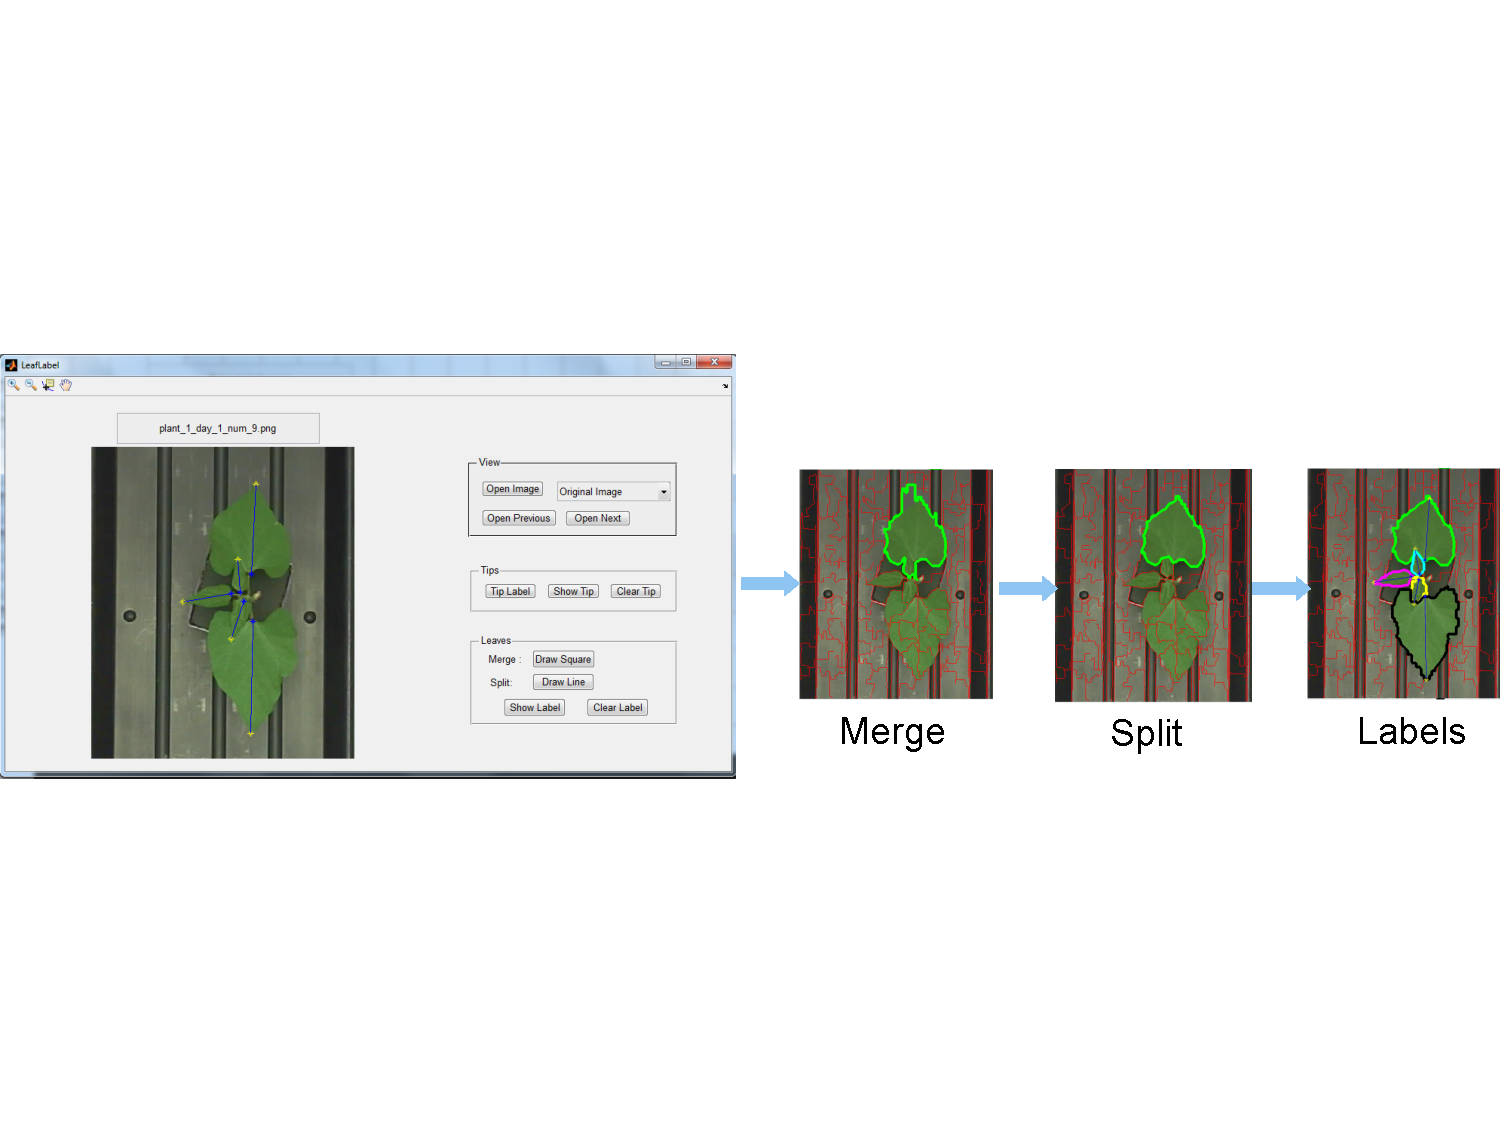
\includegraphics[width=.98\textwidth]{Figures/labeling}\\
\caption{Leaf labeling process, including tip labels and leaf annotation.}
\label{fig:label}
\end{figure*}

Tip label is implemented by clicking pairs of points on the image.
The outer tip is always clicked before the inner tip.
A line connecting each pair of tips will be shown immediately for visualization.
Inaccurate labels can be deleted by clicking the right button of the mouse near the labeled point and relabeled by clicking the left button again.

Leaf label is implemented by clicking the boundary of one leaf at each time.
The labeled leaf boundary is overlaid on the image for better visualization to guide the next action.
Incorrect label can be deleted right after the labeling.
This process continues until all leaves have been annotated.
After the labeling of one plant, we visually go through the results and correct inaccurate labels.
One example of leaf label result for one plant is shown in Fig.~\ref{fig:LabelExample}, where one color is used to represent one leaf.
As we can see, there is leaf showing up and cover up the leaf underneath, which will not be annotated later (transition between day $4$ and day $5$).

%\begin{figure}[h]
%\centering
%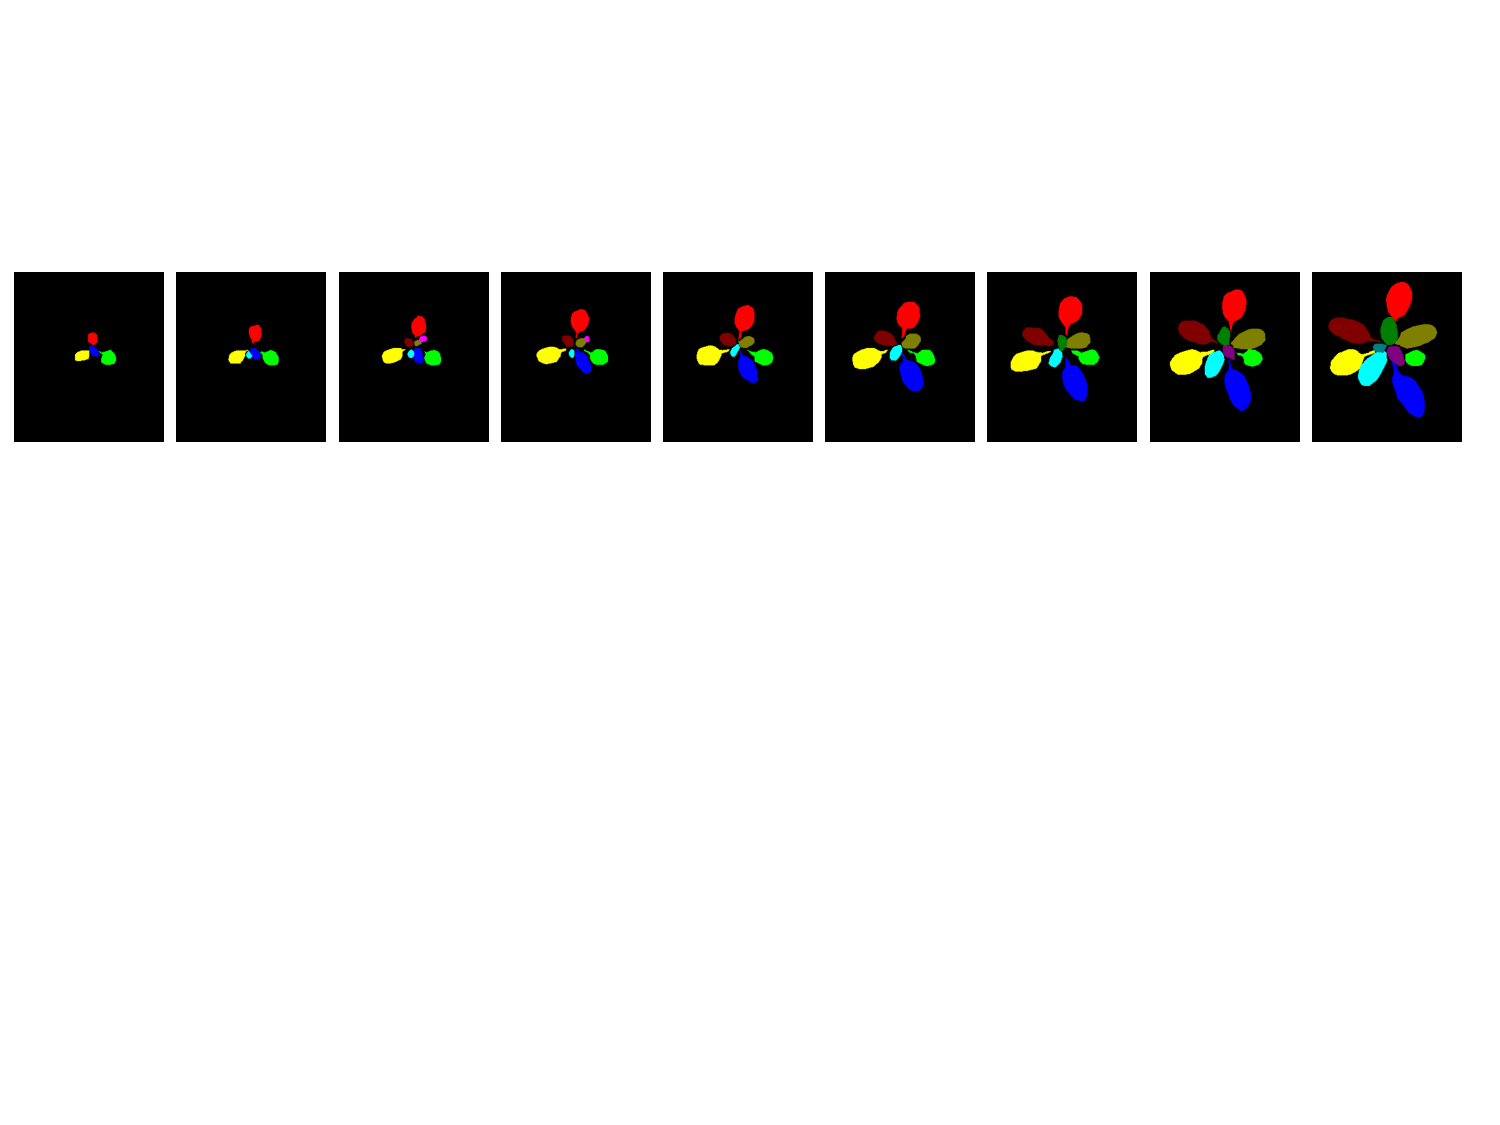
\includegraphics[width=.98\textwidth]{Figures/labelExamples}\\
%\caption{Leaf label results for one Arabidopsis plant over nine days with one image per day. }
%\label{fig:LabelExample}
%\end{figure}


\begin{figure*}
\begin{centering}
\begin{tabular}{@{}c@{} c@{} c@{} c@{} c@{} c@{} c@{} c@{} c@{}}
%\begin{tabular}{lllllllll}
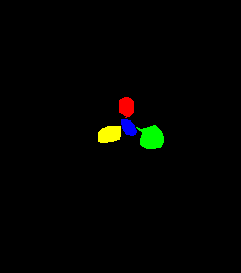
\includegraphics[width=.11\textwidth]{Figures/labelExample/plant_1_day_1_num_13.png}&
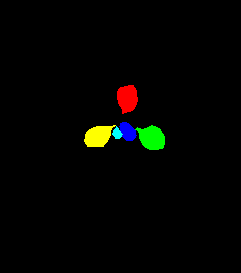
\includegraphics[width=.11\textwidth]{Figures/labelExample/plant_1_day_2_num_13.png}&
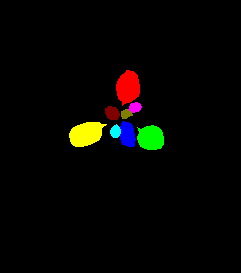
\includegraphics[width=.11\textwidth]{Figures/labelExample/plant_1_day_3_num_13.png}&
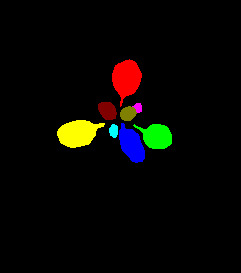
\includegraphics[width=.11\textwidth]{Figures/labelExample/plant_1_day_4_num_13.png}&
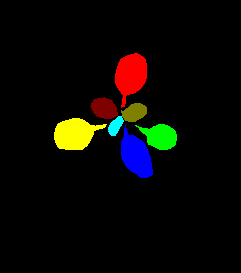
\includegraphics[width=.11\textwidth]{Figures/labelExample/plant_1_day_5_num_13.png}&
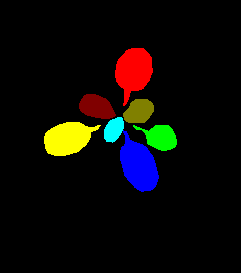
\includegraphics[width=.11\textwidth]{Figures/labelExample/plant_1_day_6_num_13.png}&
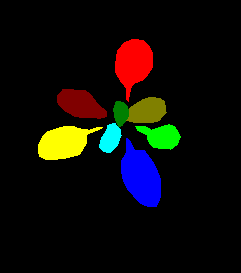
\includegraphics[width=.11\textwidth]{Figures/labelExample/plant_1_day_7_num_13.png}&
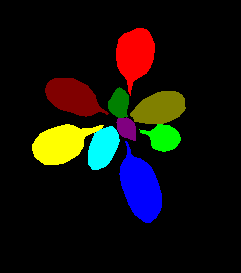
\includegraphics[width=.11\textwidth]{Figures/labelExample/plant_1_day_8_num_13.png}&
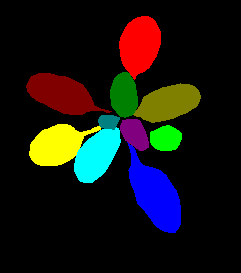
\includegraphics[width=.11\textwidth]{Figures/labelExample/plant_1_day_9_num_13.png}\\
  day 1 & day 2 & day 3 & day 4 & day 5 & day 6 & day 7 & day 8 & day 9 \\
\end{tabular}
\caption{Leaf label results for one Arabidopsis plant over nine days with one image per day. }
\label{fig:LabelExample}
\end{centering}
\end{figure*}



\subsection{File types and name conventions}
We release training and testing sets in two separate folders.
In each folder, there are two subfolders named Arabidopsis and Bean.
The files in each subfolder have the following form:
\begin{itemize}
  \item plant$\_$XX$\_$day$\_$X$\_$num$\_$XX$\_$rgb.png: the original RGB color images;
  \item plant$\_$XX$\_$day$\_$X$\_$num$\_$XX$\_$fmp.png: the original fluorescence images;
  \item plant$\_$XX$\_$day$\_$X$\_$num$\_$XX$\_$ir.png: the original IR images;
  \item plant$\_$XX$\_$day$\_$X$\_$num$\_$XX$\_$depth.png: the original depth images;
  \item plant$\_$XX$\_$day$\_$X$\_$num$\_$XX$\_$label.png: the labeled images;
  \item plant$\_$XX$\_$day$\_$X$\_$num$\_$XX$\_$tips.txt: the labeled tip locations;
\end{itemize}
where $XX$ is an integer number indicating the specific plant information.
For each image in the database, we provide four channels images in PNG files ($\_$rgb, $\_$fmp, $\_$ir, $\_$depth).
For annotated images, we have two additional files ($\_$label, $\_$tips) saving the annotation results.
Leaf segmentation results are encoded as indexed PNG files, where each leaf is assigned a unique and consistent ID over time.
Leaf ID starts from $1$ and continuously increase.
And the background is encoded as $0$.
Tips locations are saved in TXT files where each line has the following format:
\begin{itemize}
  \item leaf ID \quad tip1$\_$x \quad tip1$\_$y \quad tip2$\_$x \quad  tip2$\_$y
\end{itemize}
where leaf ID is an integer number that is consistent with the segmentation label in the PNG file.
tip1$\_$x and tip1$\_$y are floating numbers represent the coordinates of the outer tip point.
tip2$\_$x and tip2$\_$y are floating numbers represent the coordinates of the inner tip point.


In addition to the original images and annotation results, we provide another folder named Matlab with all Matlab functions that will be used for mapping between different image channels and for performance evaluation purpose.
Note that the annotation is provided based on Fluorescence images.
In order to evaluate methods developed on other channels, we provide image mapping functions between every two channels.




%For leaf annotation, we use the idea of merging and splitting super pixels.
%There are six different numbers of super pixels: $100$, $200$, $300$, $500$, $800$, $1000$.
%The user can specify which level to use depending on how well the super pixels can separate the leaves from the background.
%Because one leaf can be covered by several super pixels and one super pixel can across two leaves or the foreground and background.
%We allow merging and splitting super pixels.
%Merging is implemented by drawing a rectangle on the image.
%Every super pixel overlapping with this rectangle will be merged together.
%Splitting is implemented by drawing a line separating a leaf from the background or from another leaf.
%
%As shown in Fig.~\ref{fig:label}, several super pixels that covers one leaf are first merged together to form a large super pixel.
%Since the top part of the super pixel covers some of the background and the bottom part covers another small leaf, two lines are drawn on this super pixel to split it.
%The leaf boundary is overlaid on the image for better visualization to guide the next action.
%This process continues until all leaves have been annotated.
